\chapter{Problem domain}
\chapterintro{This chapter details mechanisms and practises that ensures a requested Quality-of-Service level is met by a means of a self-adaptive system that scales across multiple service providers.}

\section{Self-adaptive system}

\subsection{Introduction}
Guaranteeing Quality-of-Service, a critical concept in this paper, can be seen as continuous monitoring and reacting to undesirable conditions when necessary. In fact, this process is as an IT procedure and traditionally belongs to the duties of a system administrator. Figure \ref{fig:it-process} illustrates exemplary IT procedure.

\begin{figure}[!ht]
  \begin{center}
    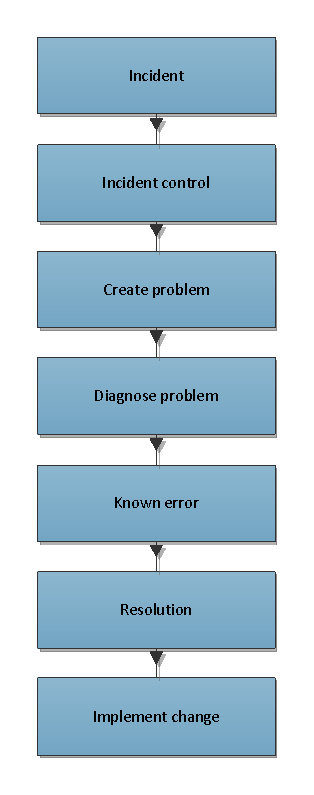
\includegraphics{chapter-adaptivity/it-process}
  \end{center}
  \caption{Exemplary IT process}
  \label{fig:it-process}
\end{figure}

While system administrator can be directly responsible for manually performing steps depicted in figure \ref{fig:it-process}, it is much more favourable to automatize this process leading to a self-manageable system. Not only does it lead to efficiency of an IT process but also to its effectiveness \cite{IBM06} achieved through:
\begin{itemize}
  \item \emph{rapid process initiation} - components auto-initiates actions based on information derived from a system
  \item \emph{reduced time and skill requirements} - automatization of IT processes makes them easier and less troublesome what is especially important for skill-intensive, error-prone and long lasting tasks
\end{itemize}

In the heart of the every self-adaptive systems, according to \cite{brun2009engineering}, lies a feedback loop, concept that originates from a control engineering. As paper's authors advocate:
\begin{quote}
Feedback loops provide the generic mechanism for self-adaptation. Positive feedback occurs when an initial change in a system is reinforced, which leads toward an amplification of the change. In contrast, negative feedback triggers a response that counteracts a perturbation. 
\end{quote}

What control loop is made of is collection of data, its analysis, making a decisions and enforcing them in the environment. Figure \ref{fig:feedback-loop} depicts a generic feedback loop, giving context associated with each phase.

\begin{figure}[!ht]
  \begin{center}
    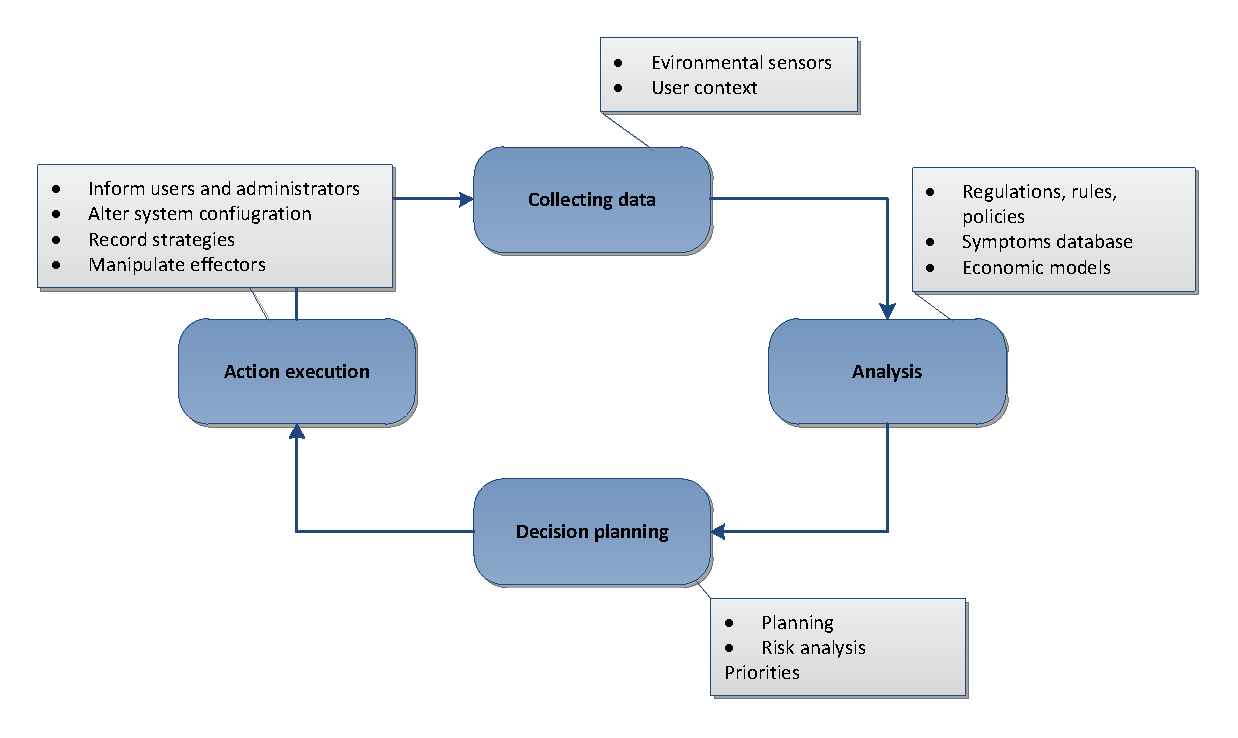
\includegraphics[width=\textwidth]{chapter-adaptivity/feedback-loop}
  \end{center}
  \caption{Feedback loop \cite{brun2009engineering}}
  \label{fig:feedback-loop}
\end{figure}

Successive sections details aforementioned phases and gives an examples of systems leveraging feedback loops.

\subsection{Collecting data}
During this phase, relevant data is collected from sensors. After that, data can be aggregated, filtered or stored to provide a reference point during future feedback loop evaluation. During this phase, there are a few concerns that should be investigated \cite{brun2009engineering}:
\begin{itemize}
 \item sample rate
 \item probe reliability
 \item data format
\end{itemize}

Almost any cloud platform providers incorporates into its solution monitoring component, responsible for data collection. Mechanisms used vary from providers to provider and may involve mixture of protocols and standards. For example, Carina \cite{Carina} uses OpenNebula IM and VMM drivers relaying on a plaintext data, transferred through a SSH connection.

\subsection{Analysis}
Analysis part applies mathematical models to reason about data gathered during previous phase. It can leverage variety of approaches and be driven by a customer-defined policies.

As \cite{brun2009engineering} specifies, it is important to take into account following concerns during analysis phase:
\begin{itemize}
 \item applying historical data and existing patterns to current situation
 \item archiving data
 \item applying adequate model to current situation
 \item model's stability
\end{itemize}

Currently, service providers employs only simplified models such as threshold model \cite{LiWoZh05}, that defines a valid range for a given metric. In cases when it is violated (i.e. value is either smaller than minimal or bigger than maximal acceptable) corresponding resource is properly adjusted - figure \ref{fig:threshold-model} illustrates that idea.

\begin{figure}[!ht]
  \begin{center}
    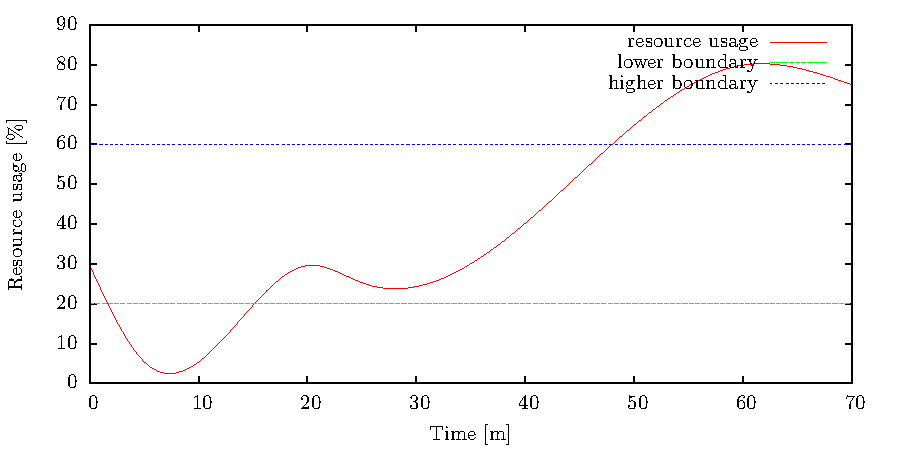
\includegraphics{chapter-adaptivity/threshold-model}
  \end{center}
  \caption{Threshold model}
  \label{fig:threshold-model}
\end{figure}

Threshold model, while trivial in its form, has been proved useful in a real-world scenarios as it is in case of AWS, OpenShift, Carina or OneCloud.

As it was already mentioned, models are often controlled by a policies that denotes a condition which, when satisfied, triggers an action, harnessing environment's disturbance. Currently, industry leaders supports \cite{AmazonAutoScaling} two kind of policies:
\begin{itemize}
 \item \textit{expression based} - allows to define how to scale application in response to changing conditions, which include factors such as memory, CPU usage, cost or some indirect, calculated metrics
 \item \textit{scheduled} - allows to scale an application in response to predictable load changes. For example, traffic increases during the weekends and decreases on working days. Hence, that predictable traffic patterns is used to scale application based on current time.
\end{itemize}

Technically, policies are expressed in a human-readable format such as JSON, XML as it is in case of AWS EC2 or custom expression used for example by Carina. Appendix \ref{app:scaling-policies} presents XML format adopted by AWS E2 Auto-Scaling.

\subsection{Decision arrangement}
Before implementing changes in an environment, decision what resources have to be tuned in order to reach a desirable state is made. Decision should be made on the basis of:
\begin{itemize}
 \item risk analysis - analysing how change effects whole environment
 \item prioritising identified problems and resources
\end{itemize}

In a case of platform-as-a-service providers, none of them explicitly specifies how a change plan is composed.

\subsection{Actions}
Finally, a change plan is implemented in a system. Actions can cover a variety of scaling and resource tuning operations. Next chapter investigates problem of scaling applications in detail.
